\documentclass[11pt]{report}

\usepackage[margin=1in]{geometry}
\usepackage{amsmath,amssymb,bm}
\usepackage{booktabs,array}
\usepackage{graphicx}
\usepackage{float}
\usepackage{siunitx}
\usepackage{natbib}
\usepackage{hyperref}
\usepackage{xr-hyper}
\usepackage[capitalise,noabbrev]{cleveref}
\usepackage{tcolorbox}
\usepackage{xparse}

\DeclareSIUnit\inch{in}
\sisetup{per-mode=symbol}

% This file lives in docs/CVT_Geometry_Notes/.
% Compile from this directory (or use latexmk -cd from the repo root).
\graphicspath{{figures/}}

% External-reference helper. Compile the main formulation once first if
% numbered links back to it are desired.
\newif\ifcinderaux
\IfFileExists{../CVT_Module_Formulation/CVT_Module_Formulation.aux}
  {\cinderauxtrue}
  {\cinderauxfalse}

\ifcinderaux
  \externaldocument[cinder-]{../CVT_Module_Formulation/CVT_Module_Formulation}
  \newcommand{\FormEq}[1]{%
    \hyperref[cinder-#1]{Equation~\ref*{cinder-#1}}%
  }
  \newcommand{\FormSec}[1]{%
    \hyperref[cinder-#1]{Section~\ref*{cinder-#1}}%
  }
\else
  \newcommand{\FormEq}[1]{\textit{main formulation equation \nolinkurl{#1}}}
  \newcommand{\FormSec}[1]{\textit{main formulation section \nolinkurl{#1}}}
\fi

% Headline-equation helpers retained from the main manuscript.
\NewDocumentCommand{\bigeq}{m m m}{%
  \refstepcounter{equation}%
  \begin{tcolorbox}
    \textbf{#2}\hfill\textbf{(\theequation)}\\[-4pt]
    \rule{\textwidth}{0.4pt}
    \[
      #3
    \]
  \end{tcolorbox}
  \label{#1}
}

\newlength{\bigeqwidth}
\NewDocumentCommand{\widebigeq}{m m m}{%
  \begingroup
  \setbox0=\hbox{\(\displaystyle #3\)}%
  \setlength{\bigeqwidth}{\wd0}%
  \addtolength{\bigeqwidth}{2em}%
  \refstepcounter{equation}\label{#1}%
  \noindent\hbox to \linewidth{\hss
    \begin{tcolorbox}[
      width=\bigeqwidth,
      boxrule=0.6pt,
      left=8pt,right=8pt,top=8pt,bottom=8pt]
      \noindent\begin{tabular*}{\linewidth}{@{\extracolsep{\fill}}l r@{}}
        \textbf{#2} & \textbf{(\theequation)}
      \end{tabular*}
      \vspace{6pt}
      \rule{\linewidth}{0.4pt}
      \vspace{8pt}
      \makebox[\linewidth][c]{\(\displaystyle #3\)}%
    \end{tcolorbox}
  \hss}\endgroup
}

\title{Supplementary CVT Geometry Notes\\
\large Belt-Length Approximation Error and Geometric Ratio Sensitivity}
\author{Kai Arseneau}
\date{\today}

\begin{document}
\maketitle
\tableofcontents

\chapter*{Scope}
\addcontentsline{toc}{chapter}{Scope}

This note preserves two pieces of CVT geometry work that are useful outside the
main CINDER manuscript but are not required to support its central transient
mechanics argument. The first quantifies the effect of a common small-angle
belt-length approximation using the current CINDER reference geometry. The
second develops geometric-ratio rate and acceleration relations and uses them
to visualize how belt length, centre distance, pulley radii, and sheave angle
shape the available ratio change.

The note is intentionally tied to the reduced belt geometry used by CINDER.
Where a result is inherited directly from the main formulation, the
\verb|\FormEq| and \verb|\FormSec| helpers link to the corresponding equation
or section in \texttt{../CVT\_Module\_Formulation/CVT\_Module\_Formulation.tex}.


\chapter{Small-Angle Belt-Length Approximation}
\label{chap:small-angle-note}

The exact CINDER belt geometry follows the outer surface of the reduced belt
path. For pulley outer-surface radii \(r_p\) and \(r_s\) and fixed
centre-to-centre distance \(C\), the exact path length is given in
\FormEq{eq:belt_length_exact}. Written here for convenience,

\begin{equation}
L_{\mathrm{geo}}
=
\pi(r_p+r_s)
+
2(r_s-r_p)\sin^{-1}\!\left(\frac{r_s-r_p}{C}\right)
+
2\sqrt{C^2-(r_s-r_p)^2}.
\label{eq:note-belt-length-exact}
\end{equation}

The installed geometry satisfies \(L_{\mathrm{geo}}=L_b\), as in
\FormEq{eq:belt_length_compatibility}. A common reduction neglects the
unequal-wrap correction when
\[
\frac{|r_s-r_p|}{C}\ll1.
\]
The resulting relation is

\begin{equation}
L_b
\approx
\pi(r_p+r_s)
+
2\sqrt{C^2-(r_s-r_p)^2}.
\label{eq:belt-length-small-angle}
\end{equation}

This chapter updates the original approximation study using the current CINDER
reference geometry and separates two different uses of
\Cref{eq:belt-length-small-angle}: inferring the installed centre distance
from a measured reference position, and using the simplified relation after the
true centre distance is already known.

\section{Approximate Centre Distance}

At a measured reference position with known \(r_p\), \(r_s\), and \(L_b\),
\Cref{eq:belt-length-small-angle} can be rearranged directly. Isolating the
straight-span term and squaring gives

\begin{equation}
C_{\mathrm{approx}}
=
\sqrt{
(r_s-r_p)^2
+
\frac14
\left[
L_b-\pi(r_p+r_s)
\right]^2
}.
\label{eq:center-distance-small-angle}
\end{equation}

The current reference configuration uses the values in
\Cref{tab:approximation-reference-geometry}.

\begin{table}[H]
\centering
\small
\renewcommand{\arraystretch}{1.12}
\begin{tabular}{@{}lll@{}}
\toprule
Quantity & Symbol & Value \\
\midrule
Outer-path belt length & \(L_b\) & \SI{0.953262}{\metre} \\
Belt radial thickness & \(h_b\) & \SI{0.0155702}{\metre} \\
Cord-layer depth & \(d_{\mathrm{cord}}\) & \SI{0.00254}{\metre} \\
Sheave half-angle & \(\beta\) & \SI{0.200712864}{\radian} \\
Primary outer radius at zero shift & \(r_{p,\min}\) & \SI{0.0362077}{\metre} \\
Secondary outer radius at zero shift & \(r_{s,\max}\) & \SI{0.1016}{\metre} \\
Deadzone boundary & \(s_{\mathrm{dz}}\) & \SI{0.0024892}{\metre} \\
Maximum shift coordinate & \(s_{\max}\) & \SI{0.01905}{\metre} \\
\bottomrule
\end{tabular}
\caption{Current reference geometry used for the approximation comparison.}
\label{tab:approximation-reference-geometry}
\end{table}

Solving the exact compatibility relation for the centre distance gives
\[
C_{\mathrm{exact}}
=
\SI{0.251616999}{\metre}
=
\SI{9.9062}{\inch},
\]
whereas \Cref{eq:center-distance-small-angle} gives
\[
C_{\mathrm{approx}}
=
\SI{0.268255528}{\metre}
=
\SI{10.5612}{\inch}.
\]

The inferred centre distance is therefore high by

\begin{align}
\Delta C
&=
\SI{0.016638529}{\metre}
=
\SI{0.6551}{\inch},
\\
\frac{\Delta C}{C_{\mathrm{exact}}}
&=
6.613\%.
\end{align}

At this reference position,
\[
\frac{r_s-r_p}{C_{\mathrm{exact}}}
=
0.2599,
\qquad
\delta
=
\sin^{-1}\!\left(\frac{r_s-r_p}{C_{\mathrm{exact}}}\right)
=
\SI{0.2629}{\radian}
\approx
\SI{15.06}{\degree}.
\]
The omitted wrap-angle correction is therefore not especially small at the
reference geometry used to infer \(C\).

\section{Propagation Along the Shift Path}

After \(C\) has been inferred, the simplified relation can also be solved
explicitly for the secondary radius. Collecting terms in \(r_s\) gives

\begin{equation}
\begin{aligned}
r_{s,\mathrm{approx}}
={}&
\frac{
\pi L_b+(4-\pi^2)r_p
}{\pi^2+4}
\\
&-
\frac{
2\sqrt{
(\pi^2+4)C^2
-L_b^2
+4\pi L_b r_p
-4\pi^2 r_p^2
}
}{\pi^2+4}.
\end{aligned}
\label{eq:secondary-radius-small-angle}
\end{equation}

The smaller physical root is used on the overdrive side. The primary outer
radius follows the current piecewise radius map in
\FormEq{eq:primary_local_radius_map}. At maximum shift,

\begin{equation}
r_p(s_{\max})
=
r_{p,\min}
+
\frac{s_{\max}-s_{\mathrm{dz}}}{2\tan\beta}
=
\SI{0.076907166}{\metre}.
\label{eq:primary-radius-at-max-note}
\end{equation}

Two ratio definitions are useful for interpreting the geometry. The
outer-surface geometric ratio used in the design maps is

\begin{equation}
R_g=\frac{r_s}{r_p},
\label{eq:outer-geometric-ratio}
\end{equation}

while the cord-line ratio relevant to the present no-slip kinematics uses
\(r_{j,\mathrm{eff}}=r_j-d_{\mathrm{cord}}\):

\begin{equation}
R_{\mathrm{eff}}
=
\frac{r_s-d_{\mathrm{cord}}}
{r_p-d_{\mathrm{cord}}}.
\label{eq:effective-geometric-ratio}
\end{equation}

At zero shift, the approximate centre distance was constructed from the same
radius pair used to evaluate the geometry. The simplified relation therefore
recovers \(r_s=\SI{0.1016}{\metre}\) exactly at that calibration point,
giving

\[
R_g=2.806033,
\qquad
R_{\mathrm{eff}}=2.942286.
\]

At maximum shift, the exact compatibility relation with
\(C=C_{\mathrm{exact}}\) gives

\[
r_{s,\mathrm{exact}}
=
\SI{0.066196036}{\metre},
\]

whereas applying \Cref{eq:secondary-radius-small-angle} with the centre
distance that was itself inferred from the small-angle approximation gives

\[
r_{s,\mathrm{approx}}
=
\SI{0.056255598}{\metre}.
\]

The resulting ratios are summarized in
\Cref{tab:approximation-ratio-errors}.

\begin{table}[H]
\centering
\small
\renewcommand{\arraystretch}{1.12}
\begin{tabular}{@{}lccc@{}}
\toprule
Configuration & Exact & Approximate & Relative error \\
\midrule
\(R_g\), zero shift
& 2.806033 & 2.806033 & 0 \\
\(R_{\mathrm{eff}}\), zero shift
& 2.942286 & 2.942286 & 0 \\
\(R_g\), maximum shift
& 0.860726 & 0.731474 & 15.02\% \\
\(R_{\mathrm{eff}}\), maximum shift
& 0.855970 & 0.722303 & 15.62\% \\
\bottomrule
\end{tabular}
\caption{Propagation of the centre-distance approximation through the current
reference geometry. The approximate column uses
\(C_{\mathrm{approx}}\) from \Cref{eq:center-distance-small-angle}.}
\label{tab:approximation-ratio-errors}
\end{table}

The large maximum-shift discrepancy is therefore not simply the local error of
dropping the wrap-angle term at that operating point. It is mainly the
consequence of first using the simplified relation to infer the wrong installed
centre distance and then carrying that distance through the rest of the shift
path.

\section{If the True Centre Distance Is Already Known}

That distinction can be checked directly. If the true installed centre
distance \(C_{\mathrm{exact}}\) is supplied to the simplified relation,
rather than inferred from it, then at maximum shift

\[
r_{s,\mathrm{approx}\mid C_{\mathrm{exact}}}
=
\SI{0.066478830}{\metre},
\]

and the corresponding cord-line ratio is

\[
R_{\mathrm{eff,approx}\mid C_{\mathrm{exact}}}
=
0.859772.
\]

Relative to the exact value \(R_{\mathrm{eff}}=0.855970\),
the error is only

\[
0.444\%.
\]

For the present geometry, then, the strongest warning concerns using the
small-angle relation to \emph{identify the installed geometry} from the
reference pulley radii and belt length. Once the true centre distance is known,
the same reduced relation is much closer over the tested maximum-shift point.

The CINDER formulation avoids both distinctions by retaining the exact
compatibility relation throughout. The numerical values in this chapter can be
regenerated with the companion script
\texttt{cvt\_geometry\_note\_calculations.py}.

\chapter{Geometric CVT Ratio Rate, Acceleration, and Design Maps}
\label{chap:ratio-geometry-note}

The CINDER geometry formulation determines the individual pulley radii and
their rates and accelerations from the shared shift motion. Those results can
also be combined to describe how the available geometric ratio changes along
the compatible pulley path.

Everything in this chapter inherits the reduced geometry used by CINDER:
fixed belt length, prescribed circular wraps and straight spans, common sheave
half-angle, and the compatible one-coordinate pulley motion. The resulting
relations and plots are therefore design tools for that reduced geometry, not
general laws for every CVT construction.

Define the outer-surface geometric ratio as
\begin{equation}
R_g=\frac{r_s}{r_p}.
\label{eq:geometric_ratio_recalled}
\end{equation}

The main formulation supplies the required pulley-radius rates in
\FormSec{sec:pulley_radius_rates} and accelerations in
\FormSec{sec:pulley_radius_accelerations}. The sections below combine those
relations and explore their geometric consequences.

\subsection{Rate of Change of the Geometric CVT Ratio}

Both the numerator and denominator in \Cref{eq:geometric_ratio_recalled} can
change with time. Using the quotient rule,

\begin{align}
\dot R_g
&=
\frac{d}{dt}
\left(
\frac{r_s}{r_p}
\right)
\nonumber\\
&=
\frac{
\dot r_s r_p-r_s\dot r_p
}
{r_p^2}
\nonumber\\
&=
\frac{\dot r_s}{r_p}
-
\frac{r_s}{r_p^2}\dot r_p.
\label{eq:geometric_ratio_rate_general}
\end{align}

The secondary-radius result in \FormEq{eq:secondary_radius_rate} supplies the
coupled secondary motion. Within the active-shift branch,

\begin{equation}
\dot r_s
=
-\frac{\phi_p}{\phi_s}\dot r_p.
\label{eq:geometric_ratio_secondary_rate_substitution}
\end{equation}

Substituting this into \Cref{eq:geometric_ratio_rate_general} gives

\begin{align}
\dot R_g
&=
\frac{1}{r_p}
\left(
-\frac{\phi_p}{\phi_s}\dot r_p
\right)
-
\frac{r_s}{r_p^2}\dot r_p
\nonumber\\
&=
-\frac{\dot r_p}{r_p}
\left(
\frac{\phi_p}{\phi_s}
+
\frac{r_s}{r_p}
\right)
\nonumber\\
&=
-\frac{\dot r_p}{r_p}
\left(
\frac{\phi_p}{\phi_s}
+
R_g
\right).
\label{eq:geometric_ratio_rate_primary_form}
\end{align}

Finally, \FormEq{eq:primary_radius_rate} gives
\(\dot r_p=\dot s/(2\tan\beta)\) in the active-shift branch. Therefore,

\bigeq{eq:geometric_ratio_rate}{Rate of Change of Geometric CVT Ratio}{
\dot R_g
=
\begin{cases}
0,
& 0\leq s<s_{\mathrm{dz}},\\[14pt]
\displaystyle
-\frac{\dot s}
{2\tan\beta\,r_p}
\left(
\frac{\phi_p}{\phi_s}
+
R_g
\right),
& s_{\mathrm{dz}}<s\leq s_{\max}.
\end{cases}
}

For an upshift, \(\dot s>0\), so the available geometric reduction decreases as
the belt moves outward on the primary pulley.


\subsection{Geometry Families in the Radius Plane}
\label{sec:ratio-plane-geometry-families}

The preceding result gives the local rate at which the geometric ratio changes
once the pulley geometry is known. To interpret that result in terms of actual
CVT design choices, it is useful to first ask which pulley-radius combinations
are available in the first place.

Recall once more that the geometric CVT ratio is

\begin{equation}
R_g=\frac{r_s}{r_p}.
\label{eq:geometric-ratio-radius-plane}
\end{equation}

Thus, every point in the \((r_p,r_s)\) plane corresponds to one geometric
ratio, and every constant-ratio contour is a line of geometrically similar
pulley states. This view is helpful because it separates three
different design questions that are easy to blur together:

\begin{enumerate}
    \item What geometric ratio does a given radius pair provide?
    \item Which radius pairs are compatible with a selected belt and installed
    geometry?
    \item How does the chosen compatible path influence the way ratio changes as
    the CVT shifts?
\end{enumerate}

The first question is answered by the constant-\(R_g\) contours. The other two
come from the belt-length compatibility relation. Once one of the global
geometric quantities---belt length \(L_b\) or center-to-center distance
\(C\)---is fixed, the compatibility relation defines a family of allowable
radius pairs in the same plane.

\Cref{fig:ratio_plane_geometry_families} compares these two views directly.
The left panel fixes the center distance and varies the belt length, while the
right panel fixes the belt length and varies the center distance. In both
panels, the solid contours are constant geometric ratio. The dashed families
are the geometrically compatible radius pairs selected by the remaining design
choice.

\begin{figure}[H]
\centering
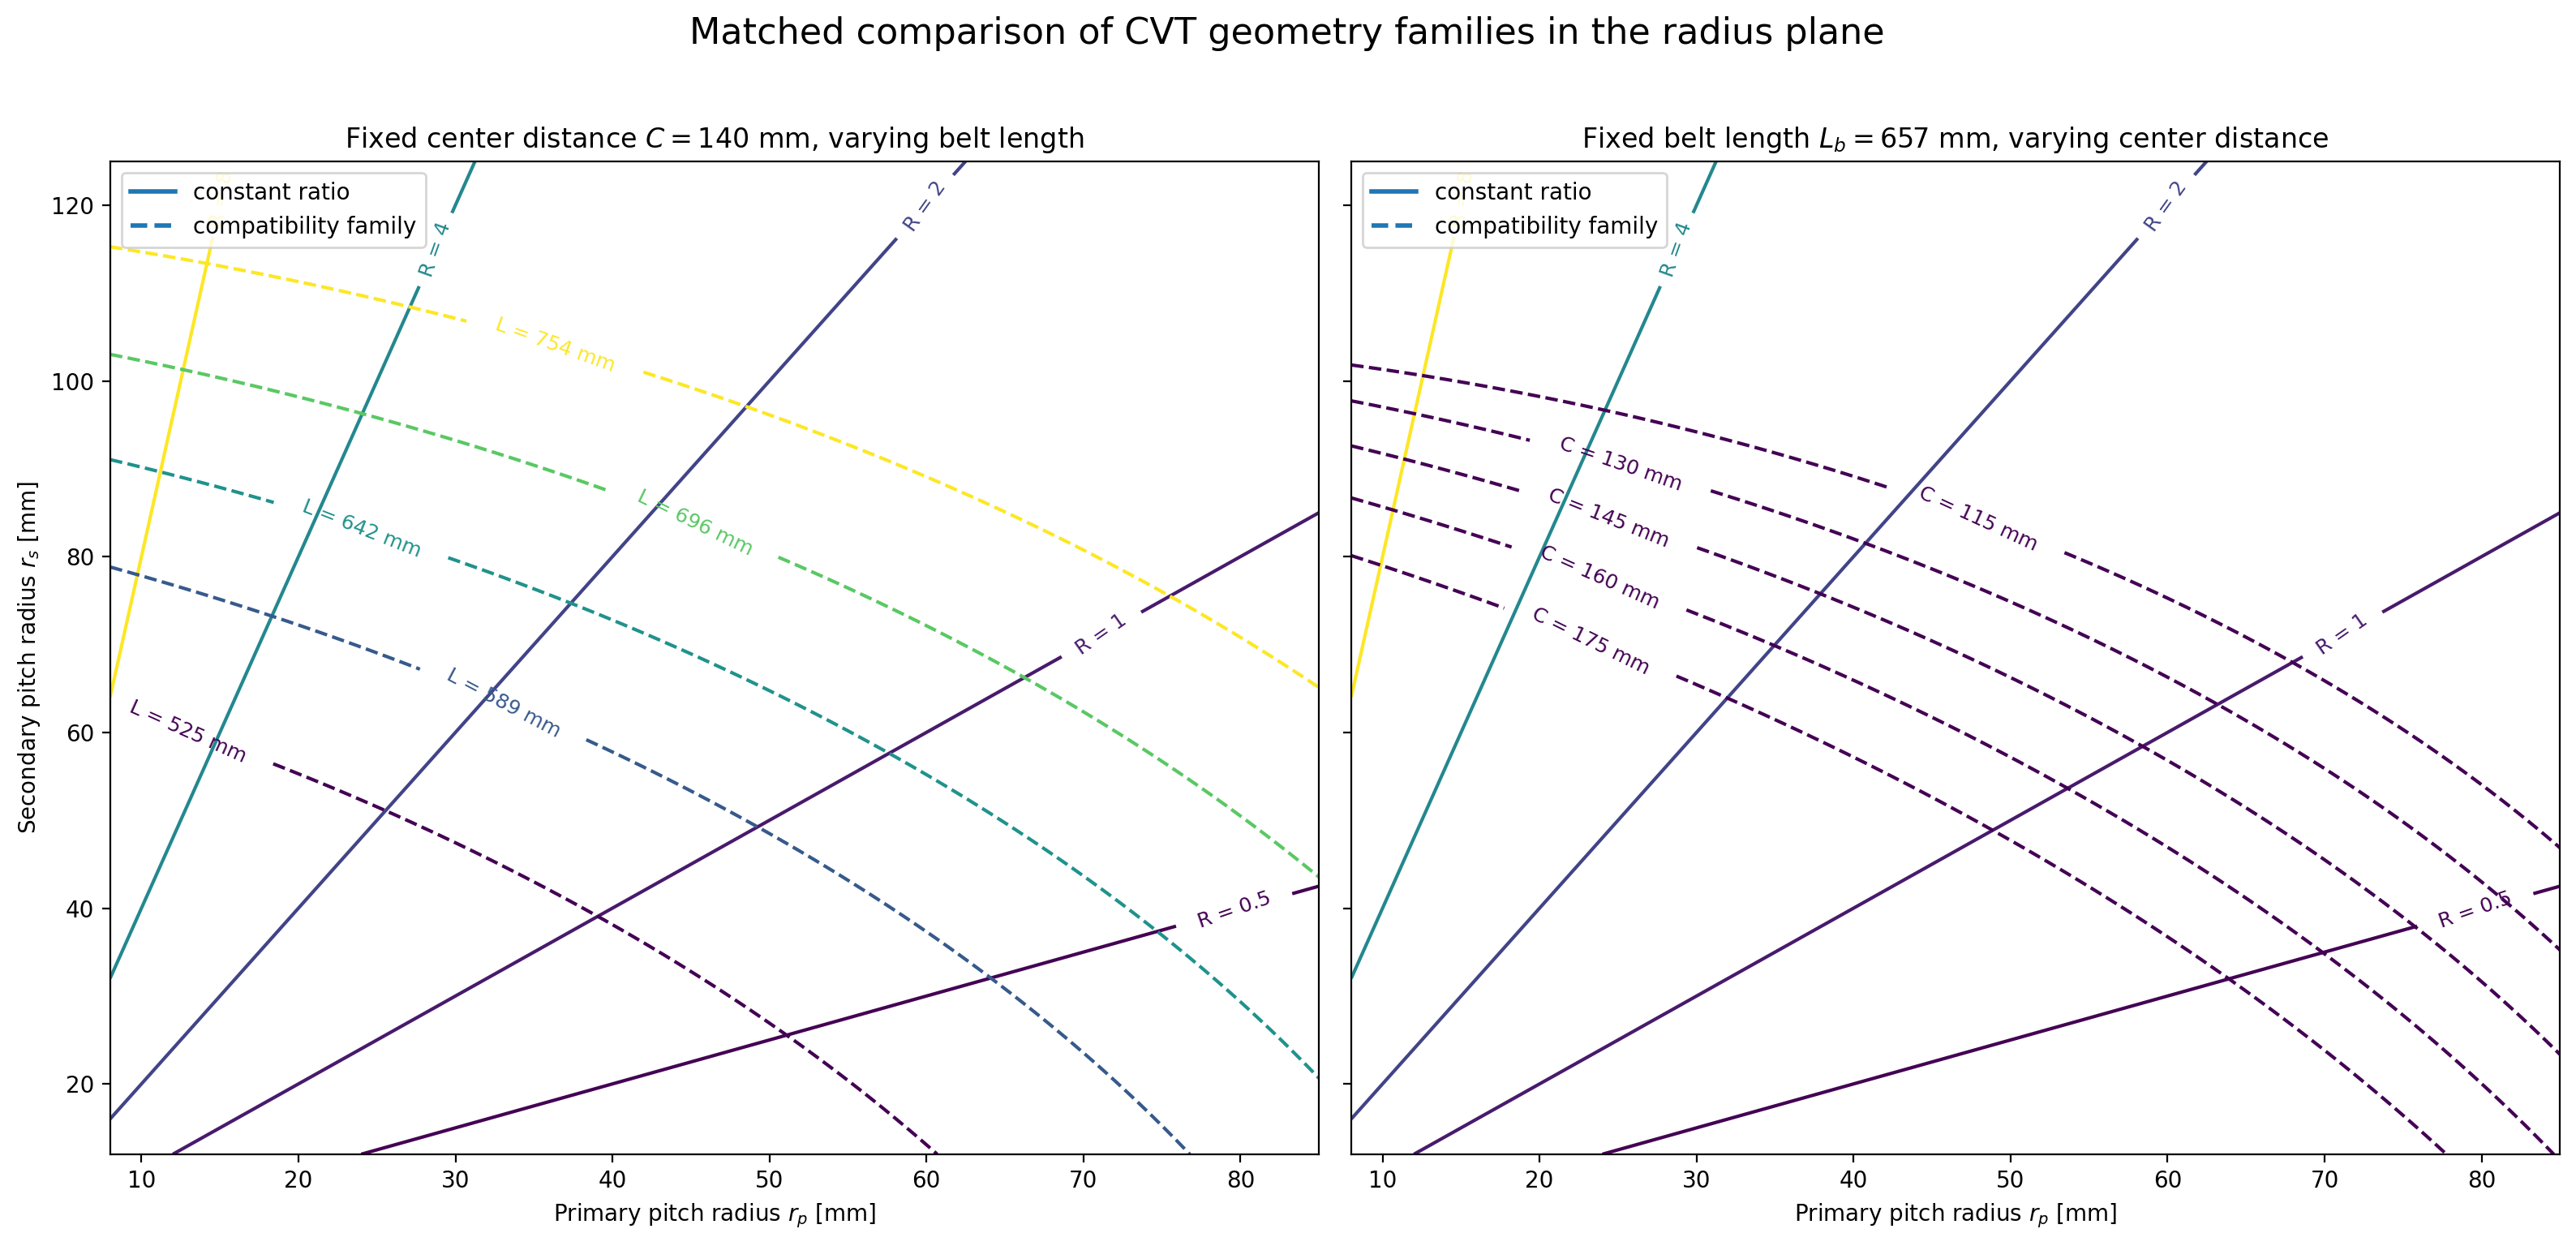
\includegraphics[width=\linewidth]{figures/cvt_geometry_matched_side_by_side.png}
\caption{
Matched comparison of geometry families in the pulley-radius plane. In both
panels, the solid contours are constant geometric ratio \(R_g=r_s/r_p\). In
(a), the center-to-center distance is fixed and the dashed families correspond
to different belt lengths. In (b), the belt length is fixed and the dashed
families correspond to different center-to-center distances.}
\label{fig:ratio_plane_geometry_families}
\end{figure}

This figure makes two points especially clear.

First, meeting a target ratio aperture is not only a matter of choosing two
endpoint ratios. The selected belt and installed geometry determine which
radius pairs are even reachable. A longer or shorter belt shifts the compatible
family through the plane, and so does a change in center distance. Since the
constant-ratio lines are not parallel to those compatibility families, changing
\(L_b\) or \(C\) changes not only the reachable endpoints, but also the
geometric route between them.

Second, the figure makes the roles of belt selection and packaging easier to
distinguish. The belt length is largely a component-selection choice, while the
center distance is largely a packaging choice. Both appear in the same
compatibility relation, but they move the admissible family in different ways.
This is why a target ratio range cannot be discussed cleanly without also
specifying either the chosen belt or the available center-to-center distance.

In this sense, \Cref{fig:ratio_plane_geometry_families} is the static geometric
view of the design problem. It shows what ratio states are available. The next
question is dynamic in a geometric sense: once the CVT moves along one of those
compatible paths, how much ratio change does a small increment of axial travel
produce?

\subsection{Exploring the Local Ratio-Change Map}
\label{sec:ratio_rate_map}

The expression for \(\dot R_g\) gives the instantaneous rate of change of the
geometric ratio. To compare different parts of the geometry without committing
to a particular time history, it is useful to divide out the shift speed and
look instead at the local ratio change produced by a small increment of axial
travel:

\begin{equation}
\frac{dR_g}{ds}
=
-\frac{1}{2\tan\beta\,r_p}
\left(
\frac{\phi_p}{\phi_s}+R_g
\right).
\label{eq:appendix_local_ratio_gain}
\end{equation}

For a small positive increment \(\Delta s\),

\begin{equation}
\Delta R_g
\approx
\frac{dR_g}{ds}\Delta s.
\label{eq:appendix_local_ratio_increment}
\end{equation}

The plots below take \(\Delta s=\SI{1}{\milli\metre}\), so the displayed
quantity may be read as the local change in geometric ratio caused by an
additional \SI{1}{\milli\metre} of primary closure. The negative sign simply
reflects the usual upshift direction: increasing \(s\) reduces the geometric
reduction ratio.

\paragraph{A sensitivity field over the radius plane}

The first view is a broad surface over the radius plane. Here, \(r_p\) and
\(r_s\) are treated as independent coordinates so that every part of the
geometry can be inspected. A real CVT does not wander arbitrarily across this
surface; its fixed belt length and center distance constrain it to one
belt-length-compatible path. Even so, the full surface is valuable because it
shows where the geometry itself makes ratio change especially strong or weak.

\Cref{fig:ratio_rate_broad_maps} shows two versions of this surface. The
unclipped view exposes the dominant trend: the local ratio change becomes much
larger in magnitude as the primary radius becomes small. This follows directly
from the explicit \(1/r_p\) factor in \Cref{eq:appendix_local_ratio_gain}, and
is reinforced by the fact that the geometric ratio \(R_g=r_s/r_p\) is also
largest in that same region. The clipped view hides the most extreme values so
that the otherwise compressed mid-range curvature can be seen more clearly. The
orange curve marks the \(R_g=1\) locus. It is a convenient reference, but not a
special boundary in the local ratio-change law itself.

\begin{figure}[H]
\centering
\begin{minipage}[t]{0.49\linewidth}
\centering
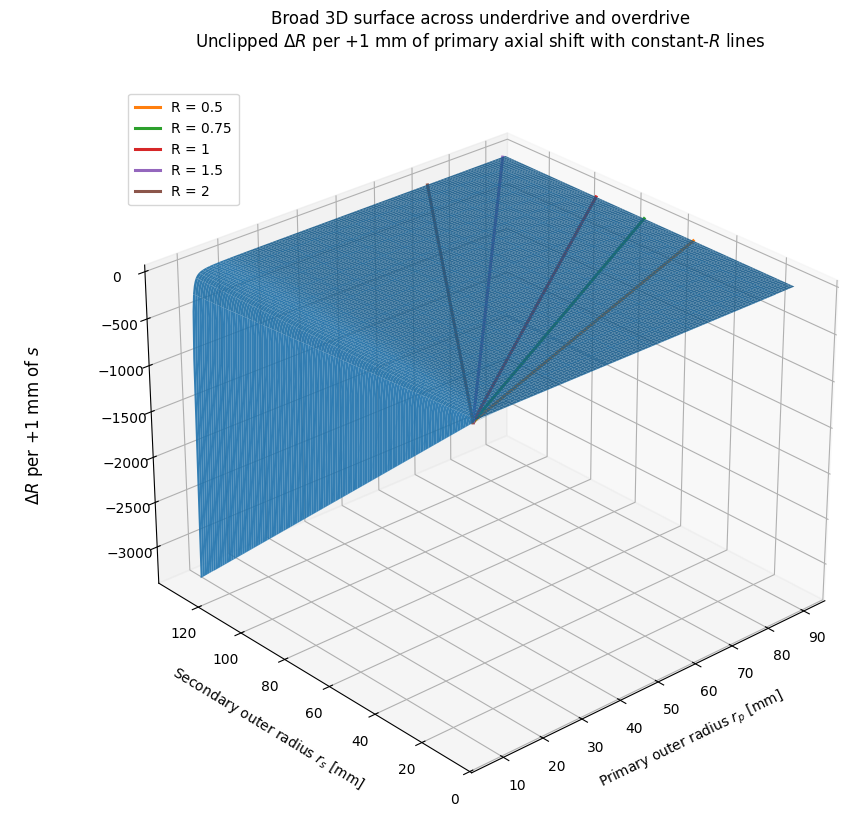
\includegraphics[width=\linewidth]{figures/zoomed_out_R.png}

\smallskip
\textbf{(a)} Broad radius domain. The full scale exposes the rapidly increasing
magnitude of local ratio change near small \(r_p\).
\end{minipage}
\hfill
\begin{minipage}[t]{0.49\linewidth}
\centering
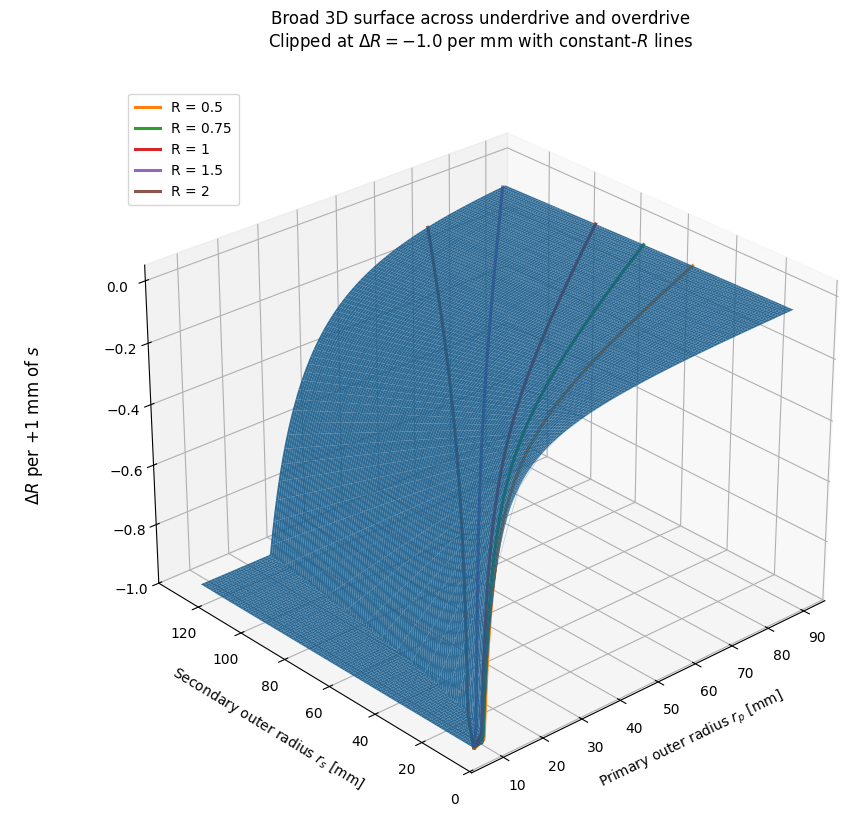
\includegraphics[width=\linewidth]{figures/truncated_R.png}

\smallskip
\textbf{(b)} The same domain with values below \(-1\) per
\SI{1}{\milli\metre} clipped, exposing the curvature through the mid-range.
\end{minipage}
\caption{
Local geometric-ratio change for a \SI{1}{\milli\metre} increase in primary
axial closure across a broad pulley-radius domain. The orange curve marks the
\(R_g=1\) locus.}
\label{fig:ratio_rate_broad_maps}
\end{figure}

\paragraph{How belt choice and installed geometry select a path}

The broad surface is useful, but a particular CVT design only experiences the
part of that field lying along its own compatible geometry path. This is where
the earlier radius-plane view becomes directly relevant. Once a belt length and
center distance are fixed, the CVT is constrained to one compatibility curve in
the \((r_p,r_s)\) plane. As the primary sheave closes, the operating point
moves along that curve and samples the local ratio-change field point by point.

\Cref{fig:ratio_rate_belt_paths} overlays three representative
belt-length-compatible paths on the local ratio-change surface. Each path
corresponds to a different belt-length/reference-geometry choice. The figure
shows that two designs with similar overall ratio aperture can still distribute
their ratio change very differently over the available shift travel. One path
may enter the steep small-\(r_p\) region early, concentrating a large amount of
ratio change into a short portion of the stroke. Another may spend more of the
stroke in the flatter region, distributing the same overall change more
gradually.

\begin{figure}[H]
\centering
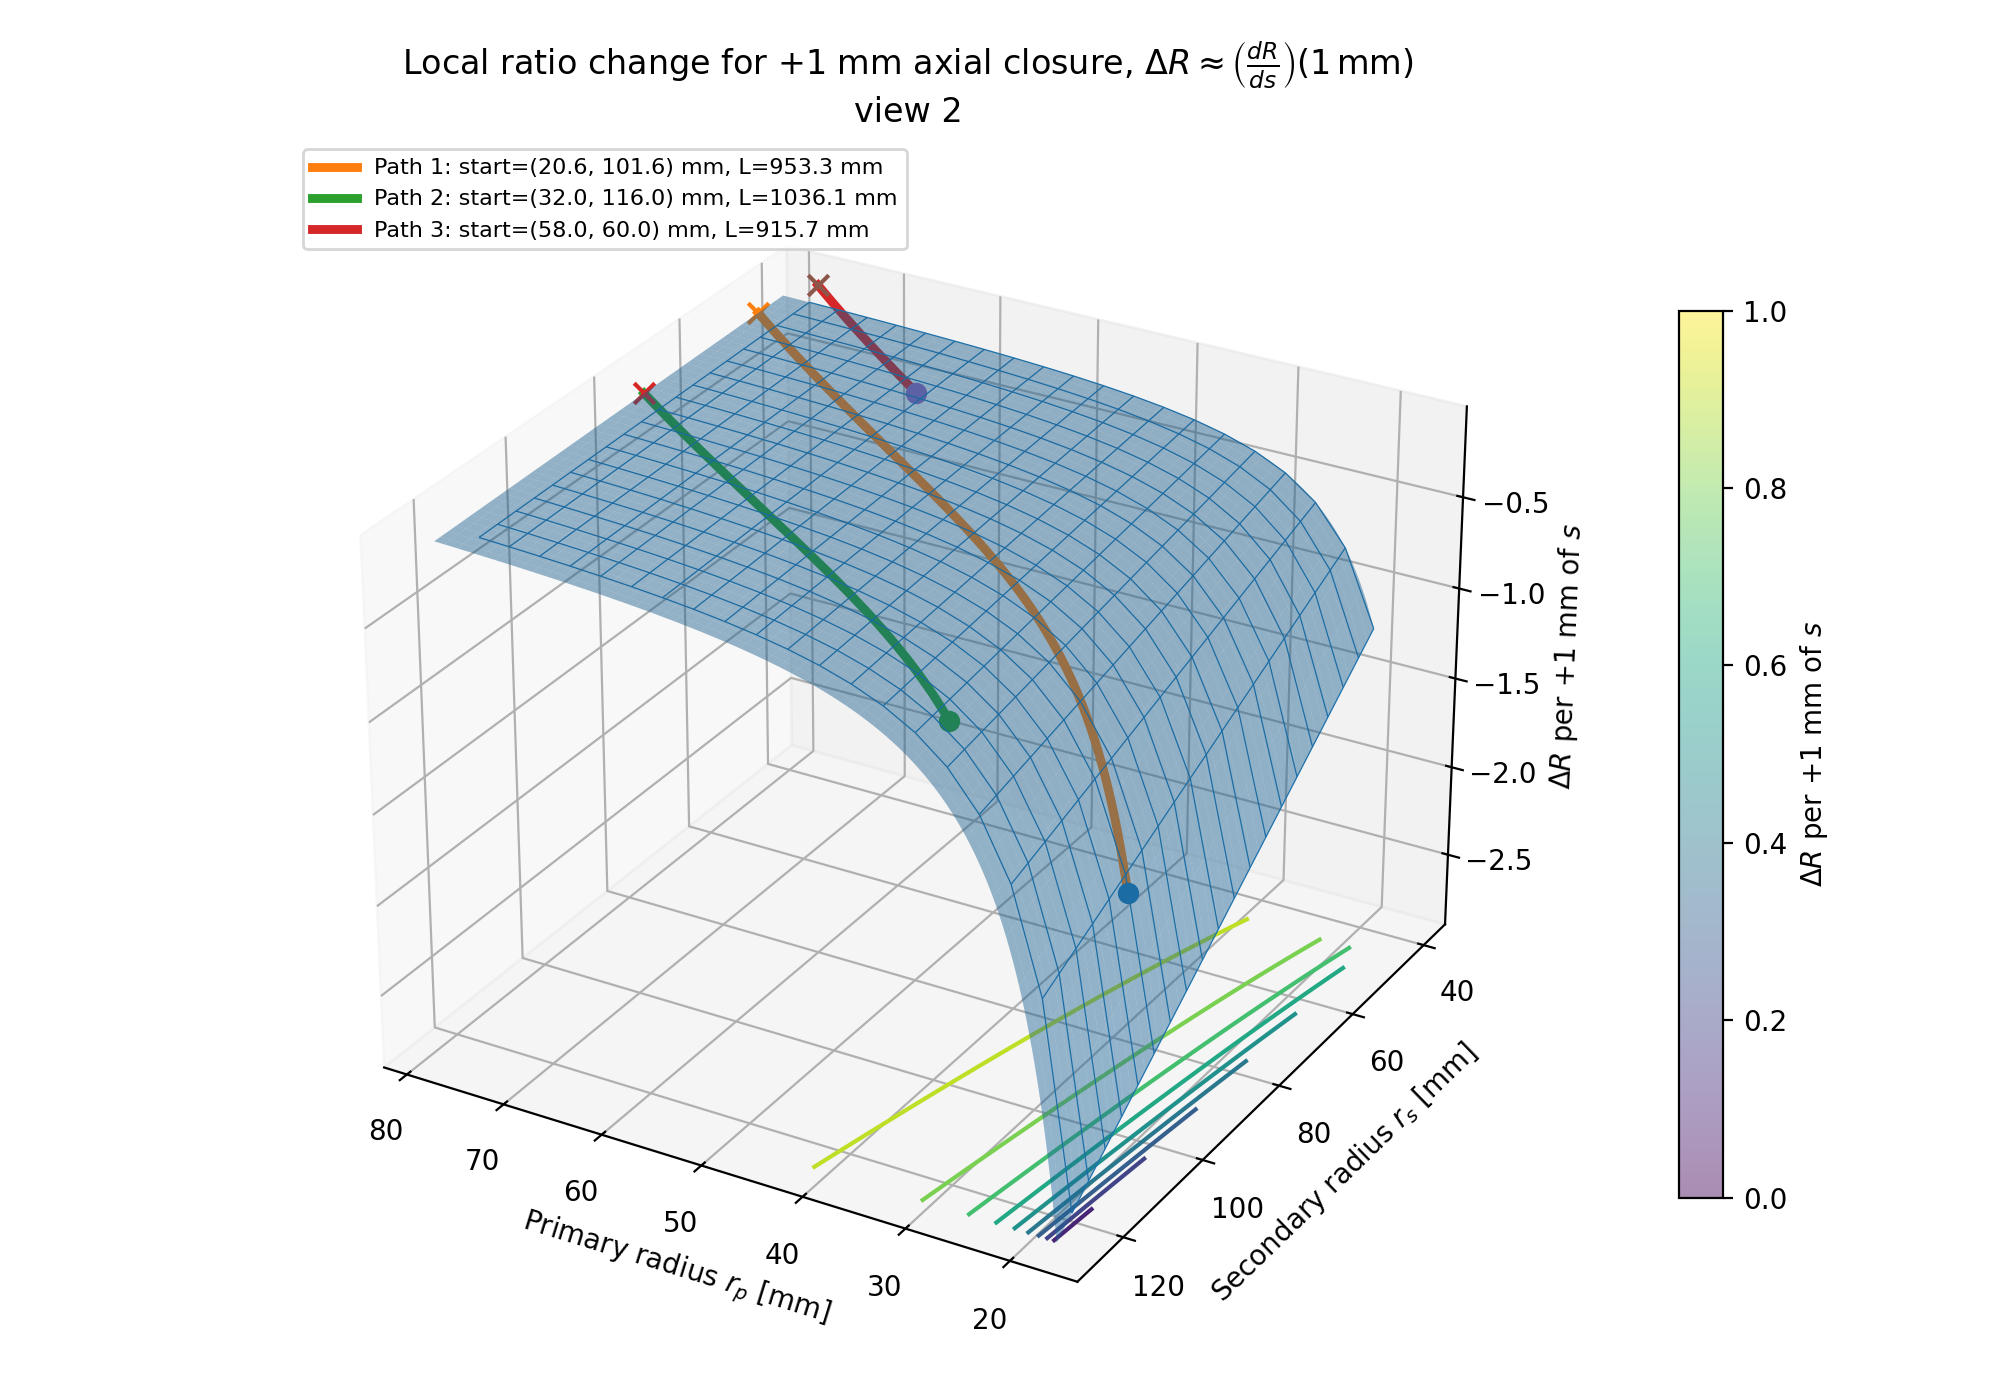
\includegraphics[width=0.90\linewidth]{figures/ratio_rate_three_belts.png}
\caption{
Representative fixed-belt-length paths through the local ratio-change surface.
Each coloured curve is a geometrically compatible pulley-radius path for a
different belt-length/reference-geometry choice. The surface value gives the
local change in geometric ratio associated with an additional
\SI{1}{\milli\metre} of primary closure at that point.}
\label{fig:ratio_rate_belt_paths}
\end{figure}

This is the key design value of the map: it does not merely say what overall
ratio range is available. It shows \emph{where along the shift stroke} that
ratio change is spent.

\paragraph{Separating the roles of the two pulley radii}

The two projections in \Cref{fig:ratio_rate_projections} help isolate the
individual effects of \(r_p\) and \(r_s\). In
\Cref{fig:ratio_rate_projections}(a), the horizontal axis is the secondary
radius and the contours identify the primary radius. For a fixed primary
radius, increasing \(r_s\) increases the geometric ratio and makes the local
ratio change more negative. The effect is visible, but the contour spacing
shows that it remains secondary to the influence of the primary radius.

\Cref{fig:ratio_rate_projections}(b) makes the primary-radius effect more
explicit. Every secondary-radius contour bends sharply downward as \(r_p\)
approaches its lower limit, then flattens at larger radius. This is the visual
form of the \(1/r_p\) dependence in \Cref{eq:appendix_local_ratio_gain}. Thus,
the small-primary-radius region is not only where the geometric reduction is
large; it is also where the ratio becomes most sensitive to additional axial
motion.

\begin{figure}[H]
\centering
\begin{minipage}[t]{0.49\linewidth}
\centering
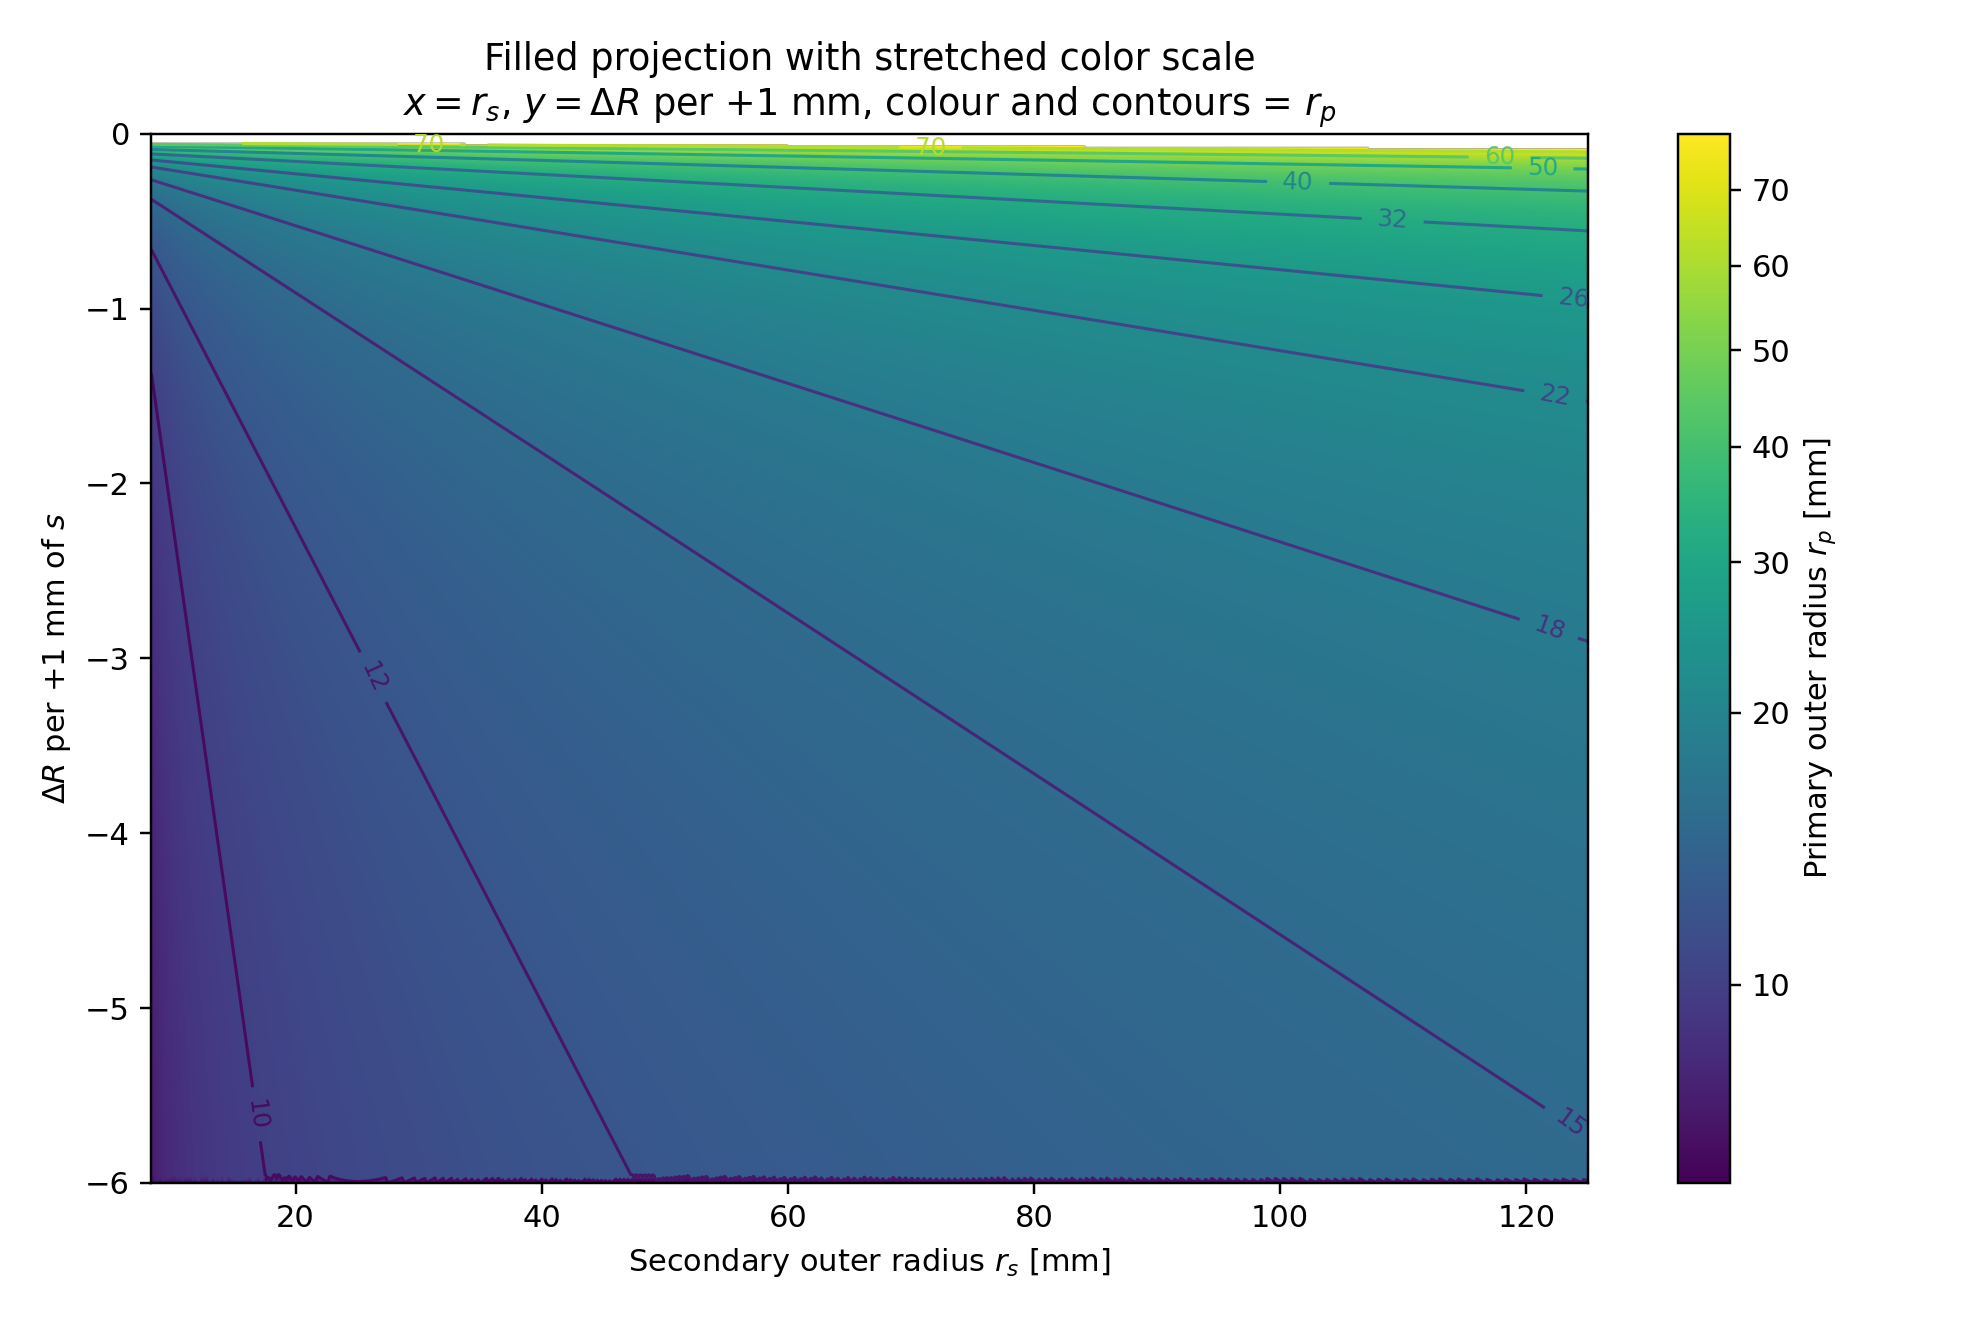
\includegraphics[width=\linewidth]{figures/r_s.png}

\smallskip
\textbf{(a)} Local ratio change against secondary radius. Colour and contours
identify the primary radius.
\end{minipage}
\hfill
\begin{minipage}[t]{0.49\linewidth}
\centering
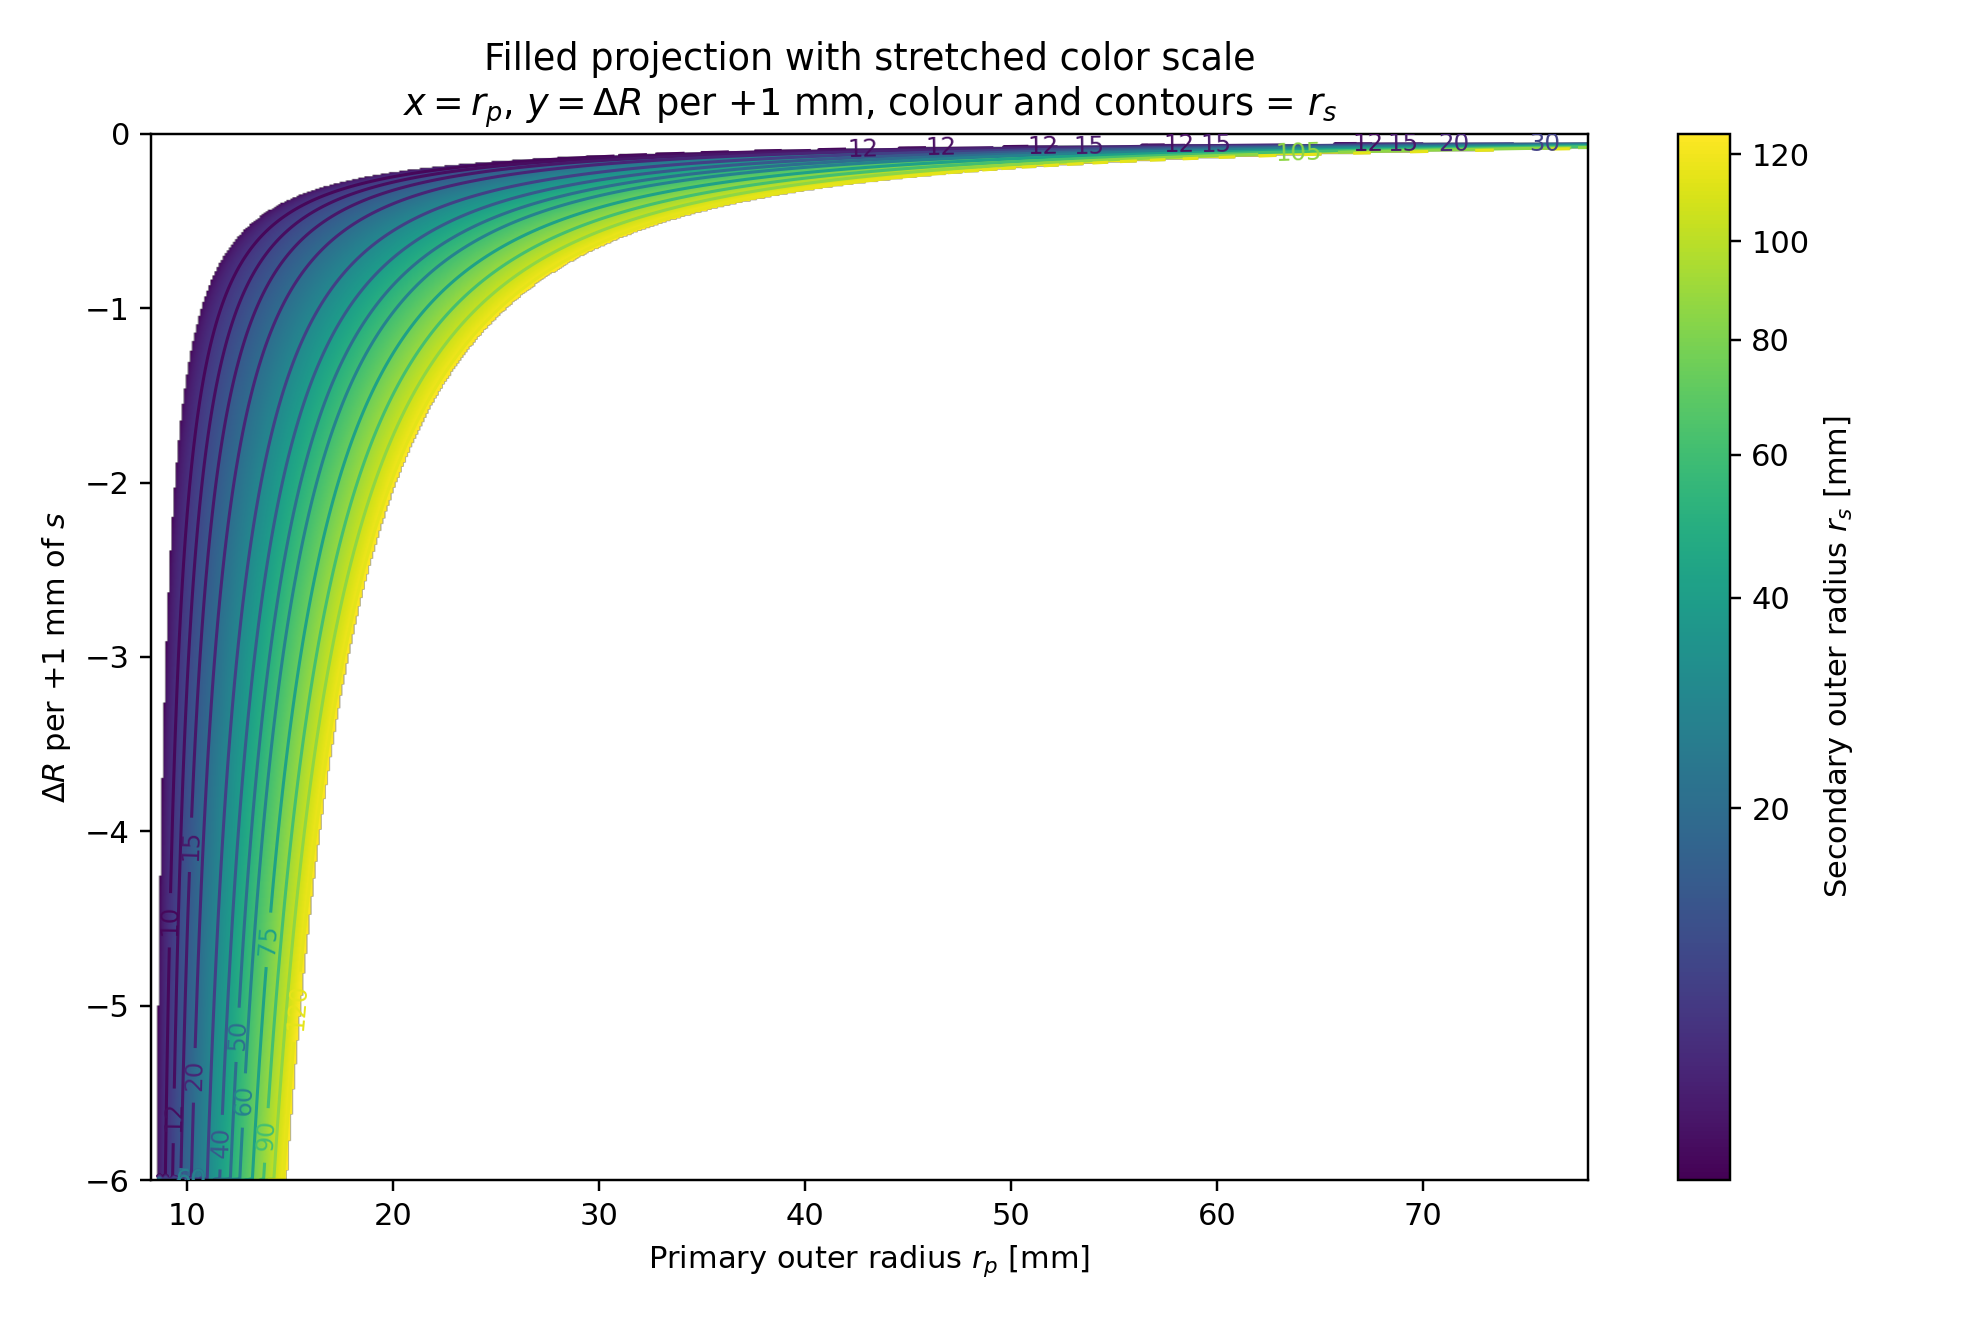
\includegraphics[width=\linewidth]{figures/r_p.png}

\smallskip
\textbf{(b)} Local ratio change against primary radius. Colour and contours
identify the secondary radius.
\end{minipage}
\caption{
Two projections of the local ratio-change surface for a
\SI{1}{\milli\metre} primary closure. The projections separate the
contributions of the two radii and show the dominant sensitivity to small
primary radius.}
\label{fig:ratio_rate_projections}
\end{figure}

\paragraph{Design interpretation}

Taken together, \Cref{fig:ratio_plane_geometry_families} and
\Cref{fig:ratio_rate_broad_maps}--\Cref{fig:ratio_rate_projections} give a more
complete geometric design picture than endpoint ratios alone.

The radius-plane view answers the question of feasibility. It makes clear how a
target ratio aperture depends on the selected belt length and the available
center-to-center distance. A longer or shorter belt can move the admissible
family enough to change both the reachable ratio range and the portion of the
plane through which the CVT shifts. Likewise, a packaging change in center
distance can move the same belt into a very different family of compatible
radius pairs.

The ratio-change view answers the question of distribution. Once a design
selects its belt and installed geometry, the compatible path through the plane
determines where ratio change is concentrated. A path that reaches very small
\(r_p\) can produce large ratio change in little axial travel, which may be
attractive when launch or climbing performance demands strong reduction with
limited shift stroke. A path that stays farther from that corner distributes
ratio change more gently and may be easier to control or to package within a
desired sheave travel.

This does \emph{not} mean that the smallest possible \(r_p\) is always best.
The present plots are geometric only. They show the leverage of the geometry,
but not its cost. Experimental work by \citet{ChenLeeSung1998} showed that, for
their rubber-belt CVT, the highest transmission efficiency occurred near a
\(1{:}1\) speed ratio, reminding us that the most attractive geometric reduction
state is not automatically the most efficient operating state. More directly,
\citet{ChildsCowburn1987b} identified additional loss penalties at small pulley
radii in V-belt drives, with belt-carcass warping and shearing proposed as
important contributors. In other words, the same small-\(r_p\) region that
offers strong geometric leverage is also the region where the belt is bent and
seated most severely.

For that reason, these plots are best used as an early design lens rather than
a final design verdict. They help screen combinations of belt length, center
distance, and pulley radii by showing not only how much ratio range is
available, but how that range is distributed over the stroke. Later traction,
loss, and dynamic analyses can then be used to judge whether the geometrically
attractive part of the design space is physically supportable
\citep{Gerbert1996,Bertini2014,Messick2018}.

\subsection{Acceleration of the Geometric CVT Ratio}

The ratio rate can change for two reasons. The primary sheave may accelerate,
and the pulley geometry continues to change as the belt moves. Differentiate
\Cref{eq:geometric_ratio_rate_general} term by term to capture both effects.

For the first term, \(\dot r_s/r_p\), use the quotient rule:

\begin{equation}
\frac{d}{dt}
\left(
\frac{\dot r_s}{r_p}
\right)
=
\frac{\ddot r_s}{r_p}
-
\frac{\dot r_s\dot r_p}{r_p^2}.
\label{eq:ratio_acceleration_first_term}
\end{equation}

For the second term, \(r_s\dot r_p/r_p^2\), all three factors may change.
Using the product rule,

\begin{align}
\frac{d}{dt}
\left(
\frac{r_s\dot r_p}{r_p^2}
\right)
&=
\frac{\dot r_s\dot r_p}{r_p^2}
+
\frac{r_s\ddot r_p}{r_p^2}
-
\frac{2r_s\dot r_p^2}{r_p^3}.
\label{eq:ratio_acceleration_second_term}
\end{align}

Subtracting \Cref{eq:ratio_acceleration_second_term} from
\Cref{eq:ratio_acceleration_first_term} gives

\begin{align}
\ddot R_g
&=
\frac{\ddot r_s}{r_p}
-
\frac{\dot r_s\dot r_p}{r_p^2}
-
\left[
\frac{\dot r_s\dot r_p}{r_p^2}
+
\frac{r_s\ddot r_p}{r_p^2}
-
\frac{2r_s\dot r_p^2}{r_p^3}
\right]
\nonumber\\
&=
\frac{\ddot r_s}{r_p}
-
\frac{2\dot r_s\dot r_p}{r_p^2}
-
\frac{r_s\ddot r_p}{r_p^2}
+
\frac{2r_s\dot r_p^2}{r_p^3}.
\label{eq:geometric_ratio_acceleration_general}
\end{align}

The current formulation gives the corresponding secondary rate and acceleration in
\FormEq{eq:secondary_radius_rate} and \FormEq{eq:secondary_radius_acceleration}. On the engaged branch, those results can be rewritten in terms of the primary radius motion as

\begin{align}
\dot r_s
&=
-\frac{\phi_p}{\phi_s}\dot r_p,
\label{eq:geometric_ratio_secondary_rate_recalled}\\[6pt]
\ddot r_s
&=
-\frac{\phi_p}{\phi_s}\ddot r_p
-
\frac{8\pi^2}
{\phi_s^3\sqrt{C^2-(r_s-r_p)^2}}
\dot r_p^2.
\label{eq:geometric_ratio_secondary_acceleration_recalled}
\end{align}

Substituting these into \Cref{eq:geometric_ratio_acceleration_general} gives

\begin{align}
\ddot R_g
={}&
\frac{1}{r_p}
\left[
-\frac{\phi_p}{\phi_s}\ddot r_p
-
\frac{8\pi^2}
{\phi_s^3\sqrt{C^2-(r_s-r_p)^2}}
\dot r_p^2
\right]
-
\frac{2}{r_p^2}
\left[
-\frac{\phi_p}{\phi_s}\dot r_p
\right]
\dot r_p
\nonumber\\
&\quad
-
\frac{r_s}{r_p^2}\ddot r_p
+
\frac{2r_s}{r_p^3}\dot r_p^2
\nonumber\\
={}&
-\frac{1}{r_p}
\left(
\frac{\phi_p}{\phi_s}
+
\frac{r_s}{r_p}
\right)
\ddot r_p
+
\left[
\frac{2}{r_p^2}
\left(
\frac{\phi_p}{\phi_s}
+
\frac{r_s}{r_p}
\right)
-
\frac{8\pi^2}
{\phi_s^3r_p\sqrt{C^2-(r_s-r_p)^2}}
\right]
\dot r_p^2
\nonumber\\
={}&
-\frac{1}{r_p}
\left(
\frac{\phi_p}{\phi_s}
+
R_g
\right)
\ddot r_p
+
\left[
\frac{2}{r_p^2}
\left(
\frac{\phi_p}{\phi_s}
+
R_g
\right)
-
\frac{8\pi^2}
{\phi_s^3r_p\sqrt{C^2-(r_s-r_p)^2}}
\right]
\dot r_p^2.
\label{eq:geometric_ratio_acceleration_primary_form}
\end{align}

Finally, use the primary radius rate and acceleration from
\FormEq{eq:primary_radius_rate} and \FormEq{eq:primary_radius_acceleration}:

\widebigeq{eq:geometric_ratio_acceleration}{Acceleration of Geometric CVT Ratio}{
\ddot R_g
=
\begin{cases}
0,
& 0\leq s<s_{\mathrm{dz}},\\[16pt]
\displaystyle
-\frac{\ddot s}
{2\tan\beta\,r_p}
\left(
\frac{\phi_p}{\phi_s}
+
R_g
\right)
+
\frac{\dot s^2}
{2\tan^2\beta\,r_p^2}
\left(
\frac{\phi_p}{\phi_s}
+
R_g
\right)
-
\frac{2\pi^2\dot s^2}
{\phi_s^3r_p\tan^2\beta
\sqrt{C^2-(r_s-r_p)^2}},
& s_{\mathrm{dz}}<s\leq s_{\max}.
\end{cases}
}

The ratio acceleration has two sources. The term proportional to \(\ddot s\)
is the direct conversion of primary-sheave acceleration into ratio
acceleration. Its magnitude is scaled by the local ratio sensitivity
\(dR_g/ds\), so the same axial acceleration produces a larger ratio response
where the geometric ratio changes rapidly with shift.

The terms proportional to \(\dot s^2\) arise even when the primary sheave moves
at constant axial speed. They reflect the curvature of the geometric relation
\(R_g(s)\): as the belt moves through the sheaves, the ratio change produced by
each additional increment of axial travel need not remain constant. In the
usual upshift direction, the large ratio sensitivity associated with small
primary radius progressively weakens as the primary radius grows. The ratio
therefore often changes rapidly at the beginning of the shift and then eases
off, even without a change in axial shift speed.



\bibliographystyle{plainnat}
\bibliography{../../refs/References}

\end{document}
